% ============================================================================ %
% Encoding: UTF-8 (žluťoučký kůň úpěl ďábelšké ódy)
% ============================================================================ %

% ============================================================================ %
\nn{Úvod}
První řádek prvního odstavce v kapitole či podkapitole se neodsazuje, ostatní ano. Vertikální odsazení mezy odstavci je typycké pro anglickou sazbu; czech babel toto respektuje, netřeba do textu přidávat jakékoliv explicitní formátování, viz ukázka sazby tohoto textu s následujícím odstavcem).

Formátování druhého odstavce. Text text text text text text text text text text text text.


% ============================================================================ %
\cast{Teoretická část}

\n{1}{Elektronické volby}
Na této stránce je k vidění způsob tvorby různých úrovní nadpisů.

\n{2}{Koncepce, výhody, nevýhody}
Text

\n{2}{Poždadvky, podmínky}
Text

\n{2}{RSA Blind Signature}
Text

\n{1}{Požadavky na funkčnost}
Níže následují ukázky vložení obrázku, tabulky a různorodých citací.


\n{2}{Obecné požadavky}

\n{2}{Specifika provozu na UTB}

\n{2}{Navrhované řešení}

\n{1}{Návrh aplikace}
Jádrem celé aplikace byl zvolen PHP framework Nette od českého vývojáře Davida Grudla. 
V konkurenci světových frameworků jako je Laravel nebo Symfony je velice oblíbený především v českém prostředí. Zcela jistě i díky kvalitní dokumentaci v češtině, pravidelným aktualizacím i aktivnímu diskuznímu fóru. 
Nette za velkými hráči rozhodně nezaostává a naopak přináší velice intuitivní způsob tvorby kvalitních, rychlých a bezpečných webových aplikací \cite{Haska2016}.

\n{2}{Architektura MVC}
Nette patří do skupiny architektonických vzorů známých jako MVC (Model View Controller), přesněji MVP (Model View Presenter). Jako první popsal MVC v roce 1979 Trygve Reenskaug pro programovací jazyk Smalltalk \cite{FowlerMVC}. Základním principem je rozdělení systému do tří samostatných částí - data jako Model a vstup a výstup jako Controller resp. View. S vývojem počítačů ustupovala potřeba tohoto dělení, jelikož jedna komponenta systému již uměla obsloužit vstup i výstup zároveň. S příchodem a~rozmachem internetu se MVC vrátilo a zatím zůstává \cite{zdrojakMVC}.

V kontextu webové aplikace chápeme Model jako data a jejich obsluhu, View jako zobrazení těchto dat uživateli a Controller zpracovává uživatelské vstupy, manipuluje s~Modelem a aktivuje View. Uživatelské rozhraní je v tomto podání tedy kombinací View a Controlleru. Současné frameworky nejčastěji kombinují vzory Front Controller (obsluha HTTP požadavku) a Page Controller (samotná logika konrétní části aplikace)~\cite{FowlerMVC}.

Variantu MVP (Model View Presenter) v současném podání popisuje Fowler\cite{FowlerPassiveView} jako vzor Passive View. Dochází k těsnější vazbě Controlleru (resp. Presenteru) a~View a~zároveň je Model izolován od View. Například v Nette neexistuje obdoba Front Controlleru, už z URL adresy totiž aplikace pozná, který Presenter i jeho metoda je volána. Logika Front Controlleru se tedy rozpustila mezi View a Page Controller, kterému se říká Presenter.

\n{2}{Nette framework}
Jak již bylo řečeno, jedná se architektonický vzor MVP. 
Jednotlivé části je potřeba chápat jako abstraktní vrstvy, nelze si pod nimi představit konkrétní (PHP) třidy.
Jedním důvodem je možné prolínání vrstev v rámci jedné třídy, tím druhým a závažnějším je pak nepochopení celého principu MVC/P architektury. Tím je myšleno domění mnohých (začínajících) programátorů, že Model je jeden konkrétní objekt (entita) \koment{zdroj - je nutny?}, přičemž modelová vrstva jsou nejen entity ale i business (nebo doménová) logika a dohromady tvoří tuto modelovou vrstvu. Pokud bude v této práci zmíněn \textbf{Presenter}, je tím myšlena konkrétní třída nebo skupina tříd nikoliv vrstva.

\n{3}{Třída Presenter}

Presenter přijímá objekt \phpinline{Nette\Application\Request}, který představuje HTTP požadavek a pomocí něho určí, jaké konkrétní metody je potřeba zavolat. 

Obrázek \ref{fig:zivotniCyklusPresenteru} přehledně popisuje sled volání jednotlivých metod, přičemž jsou všechny nepovinné. Vynecháním definic všech metod by došlo pouze k odeslání statického obsahu šablony.

\begin{figure}[h]
		\centering \tiny \fontfamily{lmtt}\fontseries{l}\selectfont
%		\def\svgwidth{0.5\columnwidth}
		\def\scgscale{1}
		\input{svg/lifecycle2.pdf_tex}
		\normalsize \sffamily
		\captionsetup{width=\linewidth}
		\caption{Životní cyklus presenteru}
		\label{fig:zivotniCyklusPresenteru}
\end{figure}
%\svgobr{Životní cyklus presenteru}{fig:zivotniCyklusPresenteru}{1}{lifecycle2}

Požadavek v Nette je tvořen kombinací \texttt{Presenter:Action}. \it{Signál} rozšiřuje základní požadavek a volá se vždy současně s aktuálním presenterem a akcí. Nejčastěji se signály využívají pro AJAXové požadavky nebo v komponentách, což jsou samostatné znovupoužitelné objekty. Samotný presenter je potomkem komponenty, z toho vyplývá, že komponenty mohou s View komunikovat napřímo pouze díky signálům. V obrázku nejsou uvedeny metody \phpinline{beforeRender()} a \phpinline{afterRender()}, které společně se \phpinline{startup()} a \phpinline{shutdown()} nemají vazbu na \it{akci} nebo \it{signál} a mohou být v~rámci Presenteru definovány právě jednou, slouží k definici společného chování napříč různými akcemi\cite{NettePresentery}.

\n{3}{Routování} \label{section:routovani}
Veškeré HTTP požadavky klienta míří na soubor \tt{www/index.php}, zde se inicialzuje prostředí Nette, požadavek se přeloží do objektu \phpinline{Nette\Application\Request} a vyvolá se příslušný Presenter. Proces překládání HTTP požadavků, resp. překlad URL se běžně u PHP frameworků označuje jako routování. Router umí URL adresu nejen rozložit ale také složit (neboli vytvářet odkazy). Maska routy říká routeru, jak přeložit URL adresu na tvar \texttt{Presenter:Action}, případně složitější tvary\cite{NetteRoutovani}. Základní instalace Nette obsahuje jednu jedinou routu, která je vidět na výňatku kódu \ref{php:simpleRoute}, tato routa převede URL tvaru \phpinline{https://domain.com/presenter/action} na požadavek tvaru \texttt{Presenter:Action}, přičemž parametr \phpinline{id} se předává jako argument metodá action a render příslušného presenteru. Pokud není v URL přítomná část presenter nebo action, doplní se o výchozí nastavení, zde \texttt{Homepage:default}. Tabulka \ref{tab:simpleRoute} obsahuje příklady překladů pomocí této základní routy.

\begin{listing}[ht]
\phpfile{tex/code/simpleRoute.php}
\caption{Základní routa v Nette}
\label{php:simpleRoute}
\end{listing}

% \tab{popisek}{label}{rozměr (0.0 - 1.0)}{definice sloupců}{obsah} 
\tab{Příklady routování}{tab:simpleRoute}{1}{ll}{
\hline
URL adresa & Nette požadavek \\
\hline
https://domain.com/ & Homepage:default \\
https://domain.com/homepage/about & Homepage:about \\
https://domain.com/article/view/12 & Article:view, id = 12 \\
}

\n{4}{Latte}
Šablonovací systém od vývojáře Nette, představuje výborné spojení s Nette. ...


\n{2}{Domain Driven Design}\label{section:DDD}
Při návrhu aplikace bylo využito zásad Domain Driven Desingu (dále též DDD), který uvedl Eric Evans ve své knize \textit{Domain-driven Design: Tackling Complexity in~the Heart of Software} \cite{EvansDDD}. Tento styl vývoje software si klade za cíl řešit návrh komplexního řešení pomocí modelu obchodní domény. Úzká polupráce klienta (\textit{doménoví experti}) a vývojářů (\textit{techničtí experti}) probíhá za pomoci společného a~jednotného jazyka (\textit{Ubiquitous Language}). Aplikace by měla být rozdělena do~několika základních vrstev a to konkrétně \cite{EvansDDD}:

\begin{itemize}
	\item \textbf{Prezentační vrstva} - přenáší informace uživateli a obsluhuje jeho požadavky.
	\item \textbf{Aplikační vrstva} - koordinuje práci ostatních objektů, neobsahuje business logiku.
	\item \textbf{Doménová vrstva} - hlavní část DDD, která obsahuje doménové objekty a~kompletní business logiku.
	\item \textbf{Vrstva infrakstruktury} - poskytuje prostředky ostatním vrstvám (komunikace, perzistence aj.).
\end{itemize}
\clearpage
Při srovnání koncepcí vrstev podle MVC/P a DDD lze říci, že se vhodně překrývají, pokud je zajištěno, že Controller neobsauje logiku doménové vrstvy. V~případě MVP pak částečně dochází k prolínání aplikační a prezentační vrstvy, což podle Evanse nehraje zásadní roli, tou je separace doménové vrstvy \cite{EvansDDD}. Dále Evans definuje základními stavební bloky doménové vrstvy následující \cite{EvansDDD}:
\begin{itemize}
	\item \textbf{Value Object} - neměnný (immutable) objekt, který reprezentuje nějakou hodnotu / vlastnost. Může to být telefonní číslo, ale i poštovní adresa skládající se z několika částí (členských proměnných).
	\item \textbf{Entity} - základní objekt, který je jednoznačně identifikován svojí \it{identitou}, jeho vlastnosti mohou být reprezentovány value objekty nebo dalšími entitami, z čehož vznikají agregáty.

	\item \textbf{Aggregate} - skupina entit, která v doméně představuje celek. \it{Root Aggregate} pak představuje vstupní bod pro okolní objekty k agregátovi. Objekty uvnitř agregátu mohou mít libovolné vazby mezi sebou, ale ne na okolní objekty. Převážná část business logiky by se měla odehrávat právě zde.
	\item \textbf{Module} - logické propojení (v kontextu domény) entit a agregátů vytváří moduly
	\item \textbf{Factory} - továrny na objekty zapouzdřují proces vytváření nových objektů. Může~to být metoda agregátu, která vytváří instance jednotlivých entit a value objektů nebo samostatná třída. Využívá se některého z návrhových vzorů Factory \cite{Vrana2013}\cite{Boehmer2015}
	\item \textbf{Service} - pokud nějaká operace nedává smysl v rámci jednoho objektu, může být zapouzdřena do samostatného objektu služby.
	\item \textbf{Repository} - získávání objektů, jejich perzistence (ukládání, mazání) je zapouzdřeno do samostatných repozitářů. 
\end{itemize}

\n{2}{Entity}\label{section:Entity}
Na základě shromážděných požadavků na aplikaci v částech \ref{section:pozadavky} a \ref{section:pozadavkyCele} byl sestaven obecný model kritických částí aplikace. Základem volební aplikace je samozřejmě model hlasování. Entita \phpinline{Election} představuje kořen stejnojmenného agregátu (\it{Aggregate Root}). Vazby mezi jednotlivými entitami jsou znázorněny jako diagram modelu v obrázku \ref{fig:ElectionModel}. Jednotlivými entitami tohoto agregátu jsou: 
\begin{itemize}
	\item \textbf{Election} - kořen agregátu představující jedny konkrétní volby / hlasování.
	\item \textbf{Question} - ve volbách představuje volenou pozici, v obecném hlasování jednu~otázku.
	\item \textbf{Answer} - množina kandidátů, resp. odpovědí na otázku.
	\item \textbf{Voter} - zahrnuje všechny oprávněné voliče.
	\item \textbf{Ballot} - všechny odevzdané hlasovací lístky v daných volbách / hlasování.
\end{itemize}

\begin{figure}[h]
	\centering
	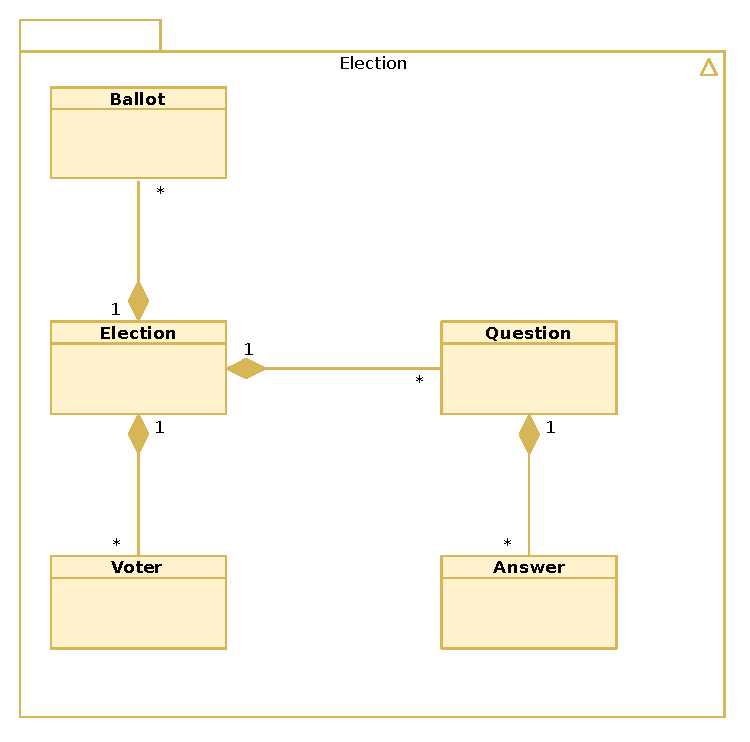
\includegraphics[width=0.6\linewidth]{svg/ElectionModelFull.eps}
	\captionsetup{width=0.6\linewidth}
	\caption[Model objektů balíčku Election]{Model objektů balíčku Election \\(zdroj: vlastní)}
	\label{fig:ElectionModel}
\end{figure}

Druhou zásadní částí aplikace je systém pro správu přístupu uživatelů (ACL). Nejjednodušší implementací takového systému je přiřazení oprávnění pomocí statické konfigurace. Tento přístup podporuje Nette bez nutnosti jakéhokoli dalšího rozšiřování o vlastní správu oprávnění. Nicméně takový přístup značně limituje flexibilitu aplikace, jelikož se jakákoli změna musí ručně zapsat do konfigurace, která bývá většinou uložena na serveru ve formě souboru. Z tohoto důvodu byl namodelován vlastní ACL systém.

\begin{figure}[h]
	\centering
	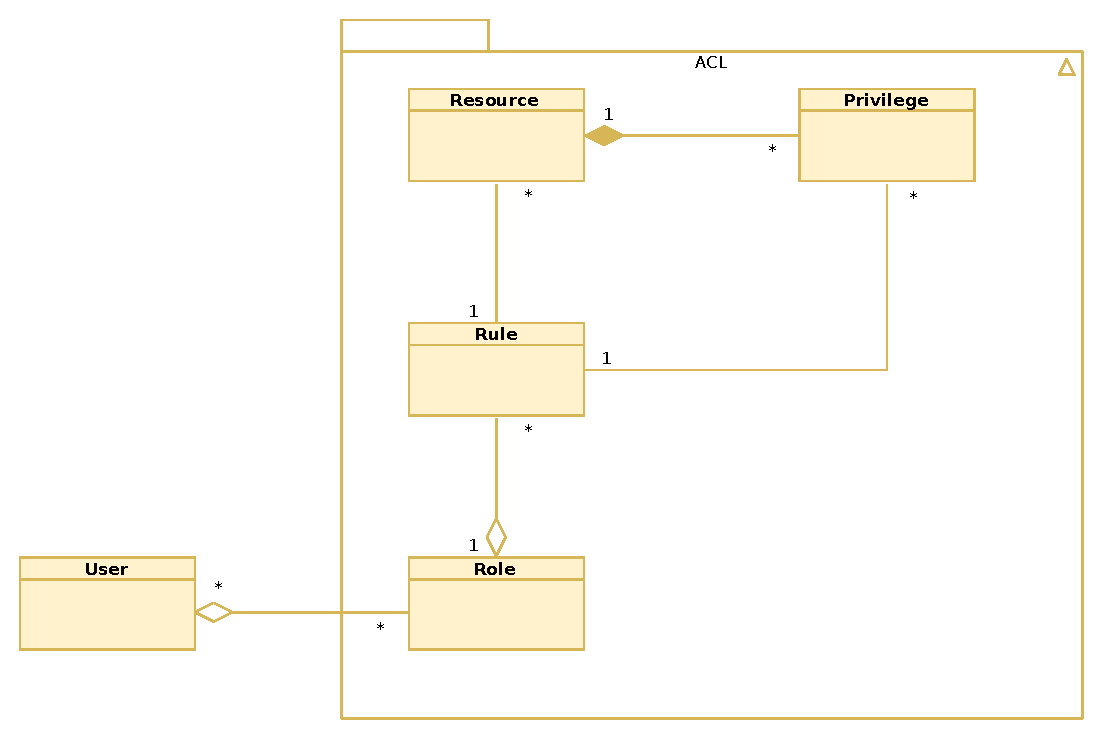
\includegraphics[width=\linewidth]{svg/ACLModelFull.eps}
	\captionsetup{width=\linewidth}
	\caption[Model objektů balíčku ACL]{Model objektů balíčku ACL (zdroj: vlastní)}
	\label{fig:AclModel}
\end{figure}
V tomto případě je kořenem agregátu entita \phpinline{Role} symbolizující jednu roli uživatele. Role může mít nastavena pravidla \phpinline{Rule}, která budou řídit přístup k~prostředkům \phpinline{Resource} a akcím \phpinline{Privilege} na nich vykonávaných. Každé pravidlo je kombinací právě jednoho prostředku a jedné akce. Pravidlo zároveň určuje, jestli je pro danou roli tato akce povolena nebo zakázána (\it{allow / deny}). Tabulka \ref{tab:prikladyACL} ukazuje příklady možného nastavení tohoto systému.


% \tab{popisek}{label}{rozměr (0.0 - 1.0)}{definice sloupců}{obsah} 
\tab{Příklady nastavení ACL}{tab:prikladyACL}{1}{llll}{
	\hline
	Role & Prostředek & Akce & Pravidlo \\
	\hline
	Student			&		Election		&		View		&	allow		\\
	Student			&		Election		&		Vote		&	allow		\\
	Student			&		Election		&		Delete	&	\bf{deny}\\
	Komise			&		Election		&		Count		&	allow		\\
	Administrator	&		Election		&		Activate	&	allow		\\
	SuperAdmin		&		User			&		Create	&	allow		\\
	\hline
}
\clearpage


\n{2}{Průchod voliče webem}
Jako další byl vytvořen zjednodušený případ užití celého systému, podle stanovanených požadavků, především s ohledem na zvolený systém anonymizace hlasovacích lístků, tak jak byl popsán v kapitole \koment{odkaz na kapitolu}.

\begin{figure}[h]
		\centering \tiny \fontfamily{lmss}\selectfont
		\def\svgwidth{1\columnwidth}
		\input{svg/ElectionUseCase2.pdf_tex}
		\normalsize \sffamily
		\captionsetup{width=\linewidth}
		\caption{Případ užití systému}
		\label{fig:UseCase}
\end{figure}

\cast{Praktická část}
\n{1}{Implementace návrhu}
Konkrétní implementace modelu popsaného v teoretické části probíhala postupně a vyvíjela se. Některé způsoby se po čase ukázaly jako nevhodné či nedokonalé a bylo potřeba je upravit resp. přepracovat tak, aby aplikace jako celek byla funkční. Během vývoje aplikace bylo změněno i IDE z Visual Studio Code na PHPstorm, což je místy vidět v rozdílných PHPdoc komentářích zdrojového kódu.

\n{2}{Členění aplikace}
Jednou ze změn, které se objevily jako vhodné v průběhu vývoje bylo rozdělení aplikace na dvě části, v kontextu Content Management Systémů běžně označované jako Frontend a Backend. Tyto dvě části by na sobě měly být nezávislé, tedy jedna nepotřebuje vědět o~(ne)existenci té druhé a umí svoje úkoly provést zcela samostatně. Frontend představuje tu část, která je veřejně dostupná, Backend označuje neveřejné administrační rozhraní aplikace. Tohoto rozdělení se zároveň využilo ke zvýšení bezpečnosti aplikace, jak je vysvětleno v části \ref{section:fyzickeOddeleni}.

Zjednodušená adresářová struktura je zobrazena v příloze \ref{priloha:adresare}. V adresáři \phpinline{app/} se nachází zdrojové kódy rozdělené podle jejich účelu. Presentery jsou společně se šablonami v příslušných adresářích (Backend, Frontend a Core). Core obsahuje presentery společné pro Frontend i Backend, což jsou momentálně pouze presentery pro zpracování chybových hlášení. Jednotlivé adresáře jsou popsány níže.
\begin{itemize}
	\item  \textbf{Backend} - obsahuje Presentery, šablony a pomocné třídy využité v Backendové části
	\item \textbf{Config} - konfigurační soubory aplikace
	\item \textbf{Core} - obsahuje Presentery, šablony a pomocné třídy využité napříč celou aplikací
	\item \textbf{Forms} - definice a továrny pro složitější formuláře
	\item \textbf{Frontend} - obsahuje Presentery a šablony využité ve Frontendové části
	\item \textbf{Models} - obsahuje modelovou vrstvu
	\item \textbf{Repositories} - všechny repozitáře pro komunikaci s modelovou vrstvou
	\item \textbf{Router} - definice routování
\end{itemize}

\n{3}{Fyzické oddělení} \label{section:fyzickeOddeleni}
Prvním krokem zabezpečení neveřejné části webu je samozřejmě omezení přístupu heslem přímo v aplikaci. Přihlašovací formulář je nicméně stále veřejný a kdokoli s~odkazem na přihlašovací stránku se může pokoušet o přihlášení. Druhým krokem tedy může být omezení přístupu pomocí IP adres (například pouze na adresy vnitřní sítě UTB) a to pomocí nastavení HTTP serveru souborem \tt{.htaccess} nebo v~konfiguraci \tt{virtualhost}. Toto nastavení je přenecháno ke zvážení tomu, kdo bude zodpovědný za instalaci a nastavení serveru.

Aby veškeré odkazy v aplikaci fungovaly a aby Nette vědělo kam má směřovat požadavky, bylo potřeba upravit základní routování popsané v části \ref{section:routovani}. Routy podporují tzv. moduly, které slouží přesně k takovému rozdělení aplikace na několik oddělených částí. Pro každý modul je možné definovat vlastní routy, seskupení rout do modulů se provádí voláním metody \phpinline{withModule(string $module)} %$ 
třídy \phpinline{RouteList}. 

\begin{listing}[ht]
\phpsnippet{tex/code/newRoute.php}
\caption{Upravená routa v Nette}
\label{php:newRoute}
\end{listing}

Rozšířené nastavení routování je patrné z fragmentu \ref{php:newRoute}. Obsahuje nastavení pro lokální testování (admin.volby.l) i simulaci produkčního prostředí na VPS serveru v~internetu (admin.volby.lukasrichter.eu). Pro Backendový modul bylo potřeba rozlišit jednotlivá prostředí podle názvu serveru kvůli použití domény čtvrtého řádu, se kterou si Router neporadil. Pro Frontendový modul toto nebylo potřeba, doména třetího řádu (volby.lukasrichter.eu) fungovala v pořádku. Zápis \phpinline{addRoute('/prihlasit', 'Sign:in')} definuje alias pro akci \tt{in} presenteru \tt{SignPresenter}, která je standardně dostupná pod adresou \tt{/sign/in}.

S tímto nastavením jsou jednotlivé části aplikace dostupné ze samostaných domén (např. admin.volby.utb.cz a volby.utb.cz), které nemusí být fyzicky na stejném serveru. Právě toto dokáže podstatně zvýšit bezpečnost aplikace. Frontendová část (volby.utb.cz) je umístěna na bežném veřejně přístupném serveru, zatímco Backendová část je umístěna na serveru, který nemusí být vůbec dostupný z~internetu. Samozřejmě může být rozdílná i samotná doména nižšího řádu, za~předpokladu, že jsou správně nastaveny DNS záznamy.

A jelikož jsou obě části na sobě nezávislé, není nutné na veřejně dostupném Frontendu umisťovat Backendový kód, který obsahuje například zpracování, dešifrování a počítání odevzdaných hlasů, ale i aktivaci a mazání celých voleb. V~případě útoku na aplikaci s cílem kompromitovat nebo ovlivnit volby, nemají útočníci možnost tento kód spustit. Museli by tedy útočit přímo na databázový server, jehož zabezpečení je v komptenci administrátora serveru.
\clearpage

\n{2}{Struktura databáze}
Celý proces získání konkrétní entity pro potřeby aplikační vrstvy je postaven na~několika návrhových vzorech. Správné užití návrhových vzorů umožní zapouzdřit chování jednotlivých tříd, nebudou vytvářena těsná propojení jednotlivých tříd a celý zdrojový kód bude flexibilnější. Cílem tohoto přístupu je zjednodušení případných budoucích úprav aplikace. Těsné provázání tříd aplikační a databázové vrstvy sice znamená méně náročnou práci při první implementaci, ale o to je náročnější kód v~budoucnosti upravit. 

Příkladem může být objekt -- entita, který se umí perzistovat, tj. je přímo závislý na~konkrétní implementaci úložiště. Při změně úložiště je pak potřeba upravit všechny takové objekty.

\n{2}{Modelová vrstva}
Z pohledu architektury MVC reprezentuje modelová vrstva data a manipulaci s nimi a v aplikaci se výrazně překrývá s doménovou vrstvou z pohledu DDD. Způsob implementace byl zvolen tak, aby zbytek aplikace nebyl pevně spojen se způsobem získávání a ukládání dat (entit).

Single Responsibility Principle (Princip jedné odpovědnosti) zavedený Robertem~C.~Martinem udává, že ``třída by měla mít pouze jeden důvod ke změně''\footnote{A class should have only one reason to change\cite{Martin2002}}. Změnou je zde myšleno přepracování kódu. Pokud má třída pouze jednu odpovědnost, pouze ta může vyvolat nutnost změny kódu. Entita má odpovědnost podávat o sobě informace, její odpovědností není, jak je vytvořena, jak a jestli vůbec je perzistována v databázi či jinde atd. Vytváření entit by měla mít na starosti třída typu \phpinline{Factory}, převedení dat z~úložiště do formátu, kterému továrna rozumí je úkolem pro \phpinline{Data Mapper}. Získání entit pro potřeby aplikace je práce pro \phpinline{Repository}. 

Získávání a manipulace s entitami byla implementována pomocí návrhových vzorů Data Mapper a Repository. Aplikační vrstva (především Presentery) získává jako závislost repozitáře (třídy typu Repository), které jí poskytují požadované entity nebo kolekce entit. V souladu se SRP Presenter nezajímá, jakým způsobem jsou entity získávány, k jeho odpovědnosti to nepatří. Repozitáře vědí, že rozhraní Data mapper umí poskytovat entity bez ohledu na to, kde a jak je konkrétní entita uložena (v paměti, souboru, databázi či jinde). V aplikaci je pouze jedna implementace a to \phpinline{DbDataMapper}. Data mapper pomocí databázového adaptéru Dibi odesílá požadavky na databázový server. Vytváření entit je řešeno částečně továrními metodami data mapperů a částečně samotnými továrními třídami v závislosti na složitosti operace. Ideální by ovšem bylo striktní oddělení do samostatných tříd.

\begin{figure}[h]
	\centering
	\includegraphics[width=\linewidth]{svg/roleMapper.png}
	\captionsetup{width=\linewidth}
	\caption[Diagram modelové vrstvy]{Diagram modelové vrstvy (zdroj: vlastní)}
	\label{fig:RoleMapper}
\end{figure}

Diagram na obrázku \ref{fig:RoleMapper} obecně popisuje použité řešení, které bylo aplikováno na všechny entity. Třída \phpinline{RoleDbMapper} implementuje rozhraní \phpinline{RoleMapper}, které je předáno třídě \phpinline{RoleRepository} jako závislost. V diagramu je použit příklad role, vyhledat ji lze podle id nebo podle vazby na entitu \phpinline{User}. Vhodné například, pokud chceme zjistit, které konkrétní role má uživatel nastaveny a tedy k jakým prostředkům a akcím má přístup díky pravidlům přiřazeným k jeho daným rolím. Zde je vhodné připomenout diagram na obrázku \ref{fig:AclModel}, který popisuje vazby mezi uživatelem, rolemi atd.

Metody \phpinline{find(), findOne(), findAll()} a \phpinline{findRelated()} slouží k vyhledání entit podle zadaných parametrů. Těmi může být filtr na Id nebo společnou vlastnost ale i vazba na jinou entitu. Metoda \phpinline{getDataSource()} slouží k získání dat pro zobrazení interaktivních tabulek v administraci aplikace. Pomocí metody \phpinline{create()} dokáže vytvořit nové instance entity \phpinline{Role}, které jsou následně předány repozitáři samostatně (\phpinline{findOne()}) nebo jako kolekce (některé mappery předávají objekt \phpinline{...Collection}, některé předávají pole objektů).
\clearpage

\n{2}{Struktura databáze}
Pomocí stanovených modelů bylo možné navrhnout podrobnější modely jednotlivých entit a tím pádem i strukturu databáze.

\begin{figure}[h]
	\centering
	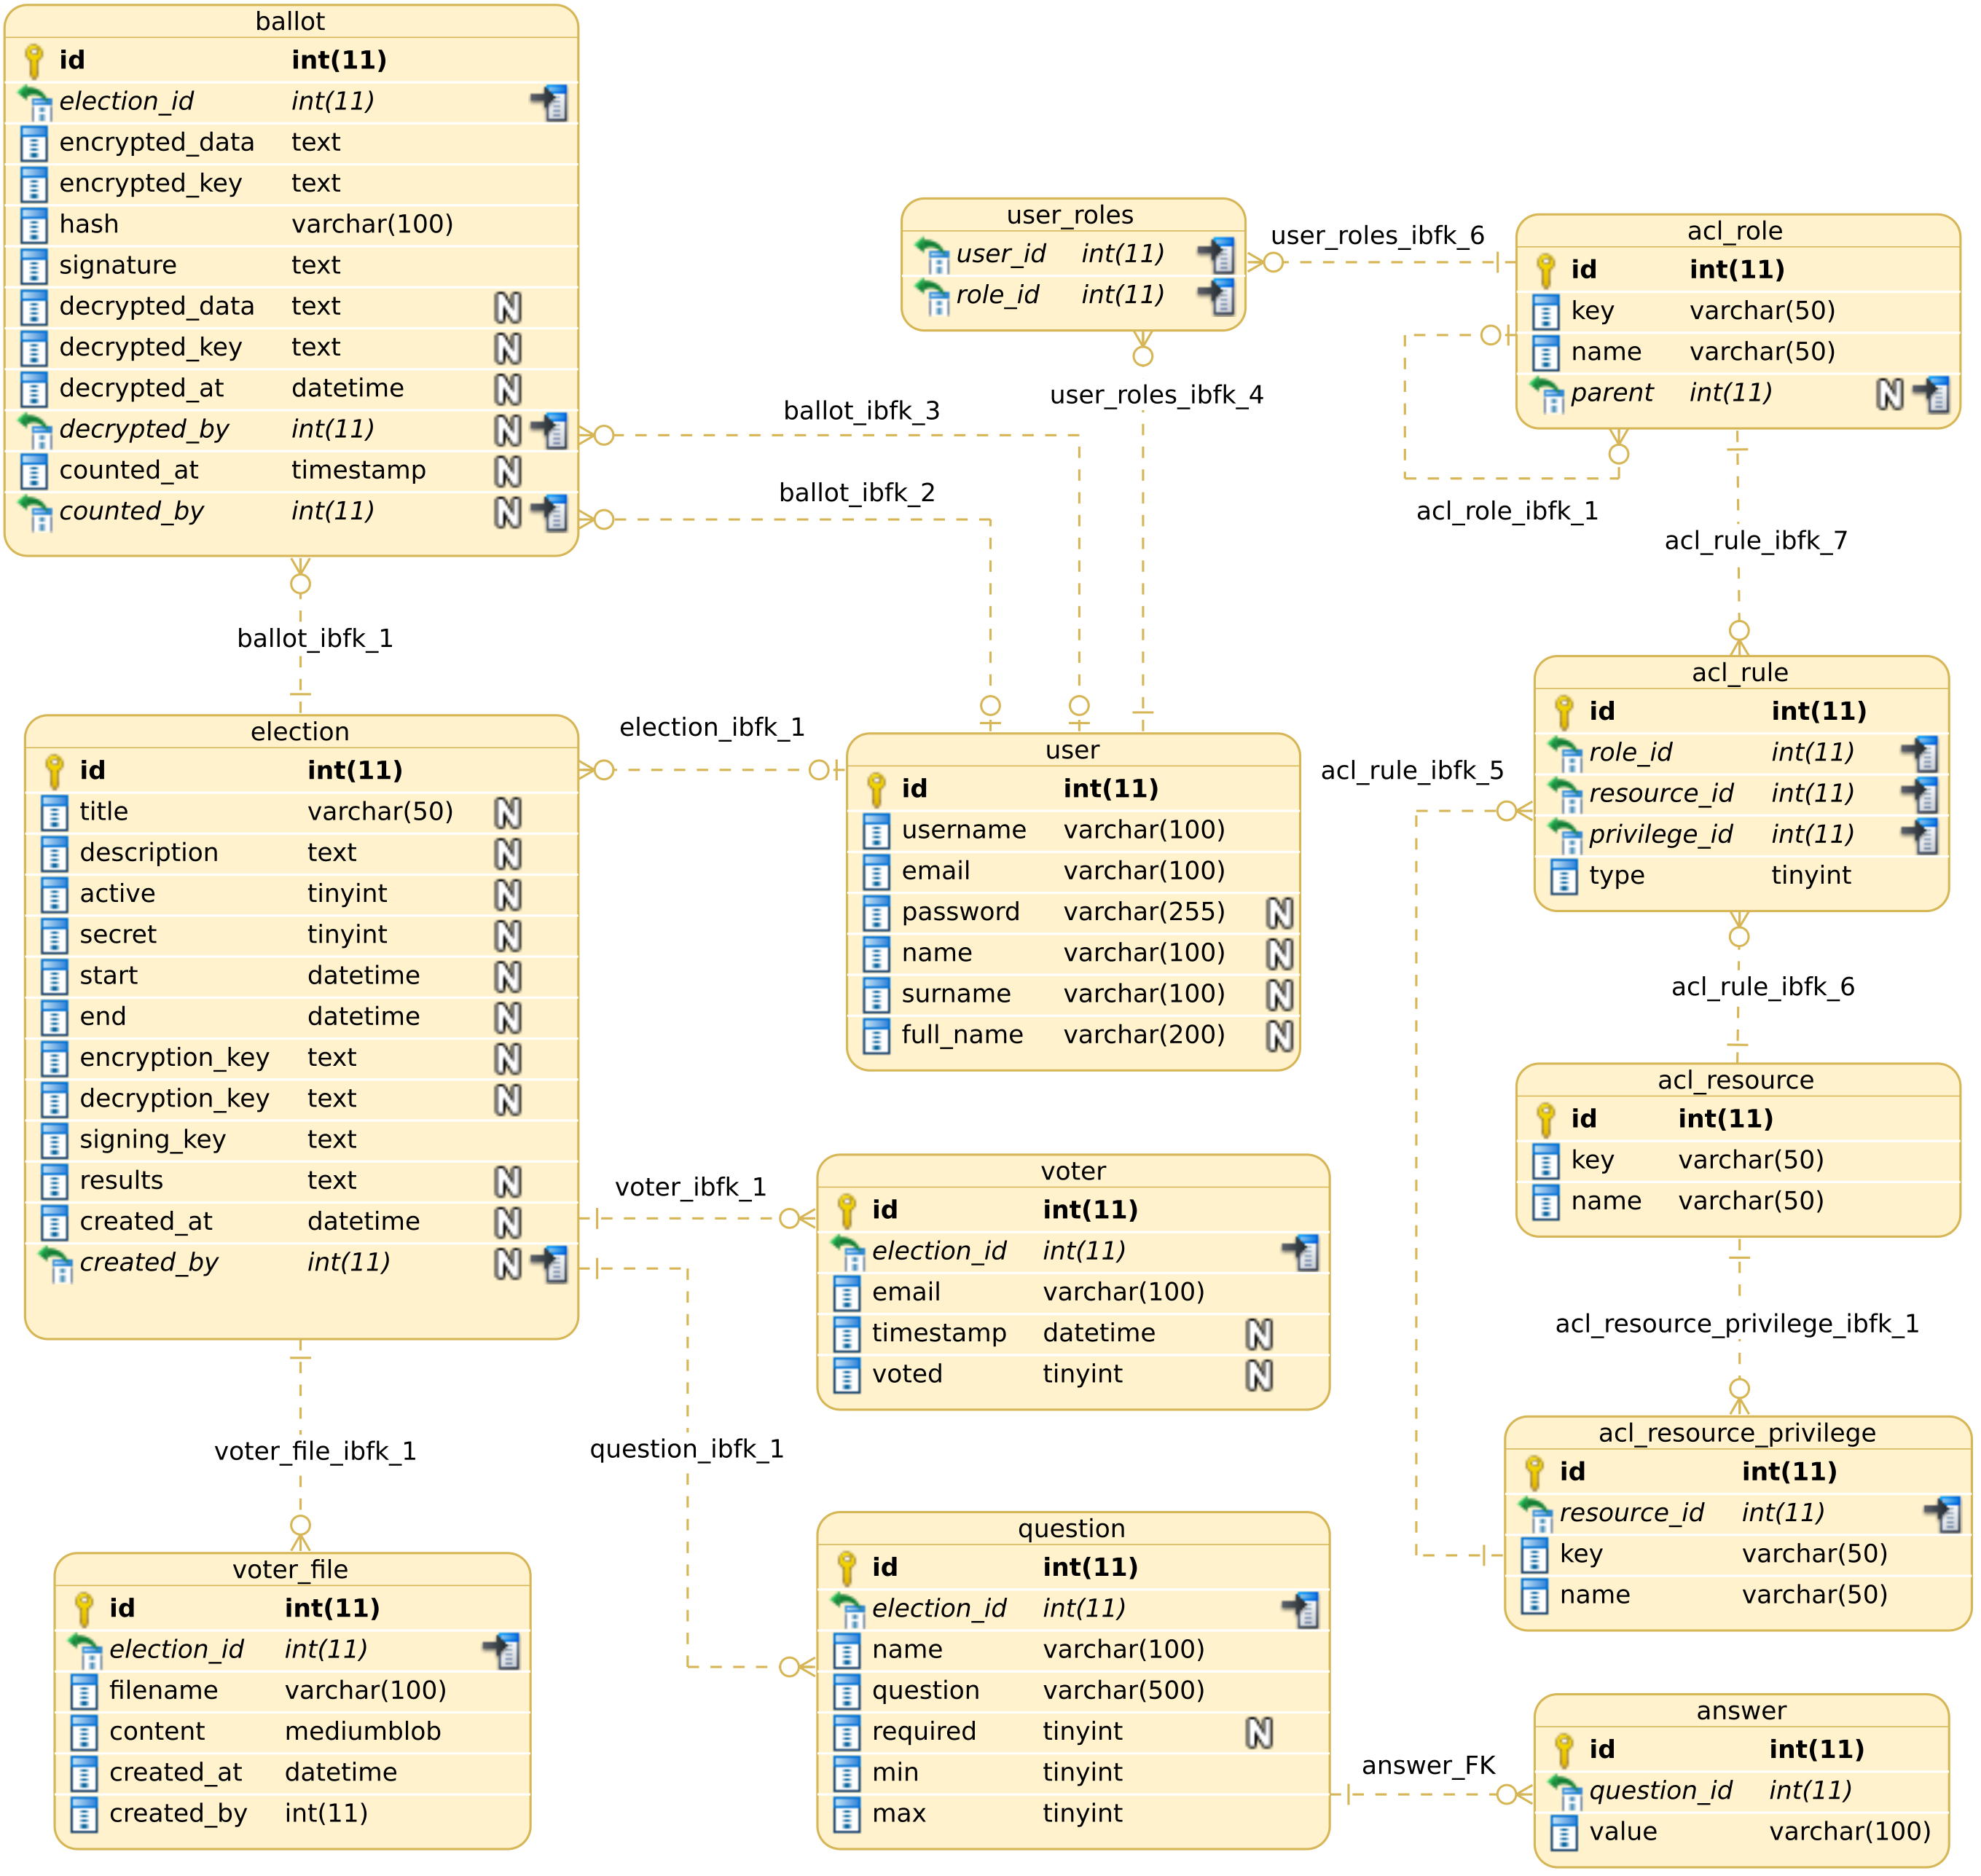
\includegraphics[width=\linewidth]{svg/erd3.png}
	\captionsetup{width=\linewidth}
	\caption[Entitně relační diagram]{Entitně relační diagram (zdroj: vlastní)}
	\label{fig:ERD}
\end{figure}


\clearpage

\clearpage
\n{2}{Přihlašovaní a autentizace} \label{section:prihlasovani}
Přihlašování uživatelů probíhá identickým způsobem pro Frontend i Backend. Aplikace je dostupná pouze pro přihlášené, pokus o přístup bez platného přihlášení vyvolá přesměrování na SignPresenter. Přestože základní URL adresa aplikace vede na \texttt{Homepage:default}, (nepřihlášení) uživatelé jsou vždy přesměrováni nejdříve na přihlašovací stránku.

K ověření (autentizaci) uživatele pomocí kombinace uživatelského jména (e-mailové adresy) a hesla v Nette slouží rozhraní \texttt{Authenticator}\footnote{\Verb{Nette\Security\Authenticator}}. Samotný proces ověření inicializuje objekt \texttt{User}\footnote{\label{user}\Verb{Nette\Security\User}}. SignPresenter po odeslání formuláře předá objektu \texttt{User} implementaci rozhraní a následně zavolá metodu \phpinline{User::login($username, $password)}. Pokud ověření selže, je vyvolána výjimka \texttt{AuthenticationException}, která je zachycena v presenteru. Úspěšná autentizace způsobí uložení implementace \texttt{IIdentity} do objektu \texttt{User}.

Jedním z požadavků na aplikaci byla stanovena možnost přihlášení voličů pomocí univerzitních e-mailových adres. Implementace ověřování metodou Single Sign-On přes systém Shibboleth by byla nad rámec této práce a po diskuzi s vedoucím práce bylo zvoleno ověřování pomocí Active Directory přes LDAP. Dalším požadavkem byla možnost přihlášení externích uživatelů bez nutnosti vytvářet jim univerzitní e-mailové adresy. Tohoto bylo docíleno možností ověření vůči databázi aplikace.

\begin{listing}[ht]
\phpsnippet{tex/code/autentizace.php}
\caption{Autentizace v SignPresenter}
\label{php:autentizace}
\end{listing}

K autentizaci se využívají dvě implementace třídy \texttt{Authenticator}. První se k ověření použije \texttt{PasswordAuthenticator}, která při úspěšném ověření vrací entitu uživatele včetně všech rolí, při neúspěchu následuje pokus o ověření přes \texttt{LdapAuthenticator}.

\begin{itemize}
	\item \textbf{PasswordAuthenticator} v prvním kroku získá na základě e-mailové adresy entitu uživatele z repozitáře. Pokud takový uživatel v databázi není, je vyvolána výjimka \texttt{AuthenticationException}. V druhém kroku předá uloženou hash hesla a ověřované heslo třídě \phpinline{Nette\Security\Passwords} k porovnání. Pokud heslo neodpovídá, je opět vyvolána výjimka. Úspěšné ověření vrátí získanou entitu.
	\item \textbf{LdapAuthenticator} v prvním kroku se pokusí ověřit kombinaci e-mailové adresy a hesla vůči univerzitnímu Active Directory, při neúspěchu vyvolá výjimku. V druhém kroku se pokusí získat z repozitáře entitu uživatele s odpovídající e-mailovou adresou, pokud takový neexistuje, je vytvořena nová entita s rolemi získanými z Active Directory. Tyto role jsou buď \textit{Student} nebo \textit{Zaměstnanec}.
\end{itemize}



\clearpage
\n{2}{Oprávnění a autorizace}
Ověření oprávnění uživatele provést akci (autorizace) na frontendové části je velice přímočaré. Zobrazit přehled aktivních voleb může kdokoli úspěšně autentizovaný systémem. Volit a zobrazit výsledky může kdokoli, kdo je uveden na seznamu voličů. Není třeba provádět žádnou dodatečnou autorizaci operací.

Backendová část je v tomto ohledu o něco složitější. Jednotliví uživatelé mohou mít přístup k presenteru, ale už ne k nějaké jeho konkrétní akci nebo signálu (metodám obecně). Podle modelu definovaného v části \ref{section:Entity} byly vytvořeny jednotlivé třídy entit. Proces autorizace stejně jako autentizace inicializuje Nette objekt \texttt{User}\footnote{\label{user}\Verb{Nette\Security\User}}. V případě přihlašování uživatelů jsou mu předávány implementace napřímo, jelikož se používají dvě různé. U autorizace stačí předat jednu konkrétní implementaci, což je nejjednodušší provést v konfiguračním souboru aplikace. V soubrou \texttt{common.neon} tedy byly zaregistrovány služby \texttt{Permission}\footnote{\Verb{Nette\Security\Permission}} a \texttt{AuthorizatorFactory}. Framework se o předání závislostí postará sám.

V rámci třídy \texttt{AuthorizatorFactory} jsou z repozitáře získány včechny prostředky a jejich akce a zaregistrovány v \texttt{Permission}. Dále se získají všechny role a postupně se zaregistrují společně s jejich pravidly. Jako poslední je zaregistrována role \textit{superAdmin}, uživatel s touto rolí má nastaveno jediné pravidlo - vše povoleno. 

\begin{listing}[ht]
\phpsnippet{tex/code/autorizace.php}
\caption{Tovární metoda třídy AuthorizatorFactory}
\label{php:autorizace}
\end{listing}

Nette umožňuje pravidla nastavovat dvojím způsobem, výčtem povolených akcí a~povolením všech akcí a výčtem akcí zakázaných. Aplikace umožňuje vytvořit pravidla obou typů, zakazující (deny) typ má nicméně smysl pouze pro roli superAdmin, která je jako jediná definována druhým způsobem. Ostatní role vždy obsahují pouze výčet povolených akcí, vše ostatní je zakázáno.

Zjistit, zda je uživatel oprávněn provést požadovanou akci, lze několika způsoby. Napřímo pomocí metody \phpinline{User::isAllowed($resource, $privilege)}, která vrací \texttt{true}, pokud alespoň jedna z rolí uživatele k akci opravňuje, jinak vrací \texttt{false}. Tento způsob lze využít i v šablonách, kde je objekt uživatele automagicky [\textit{sic}] dostupný jako proměnná \phpinline{$user}%$
. V presenterech se získá pomocí \phpinline{$this->getUser()} %$
 a~komponenty mají presenter dostupný jako členskou proměnnou, objekt \texttt{User} tedy získají pomocí \phpinline{$this->presenter->getUser()}%$
. Ostatním třídám aplikace se předává jako závislost v konstruktoru pomocí DI Containeru.

Jelikož presentery zpracovávají především požadavky od uživatele, podstatná část jejich metod by obsahovala opakující se volání metody \texttt{isAllowed}. Proto bylo využito anotací jednotlivých metod, příklad takové anotace je uveden ve fragmentu \ref{php:autorizaceAnotace}. Čtení anotací Nette usnadňuje pomocí objektu \texttt{MethodReflection}\footnote{\Verb{Nette\Application\UI\MethodReflection}}, který je předáván metodě \texttt{checkRequirements()} každého presenteru. Tato metoda je v průběhu životního cyklu presenteru volána několikrát, poprvé při jeho vytvoření a předává se jí objekt \texttt{ComponentReflection}\footnote{\Verb{Nette\Application\UI\ComponentReflection}} - reflexe aktuálního presenteru - a poté před každým \textit{action}, \textit{handle} a \textit{render} v tomto pořadí s reflexí dané metody. Tímto bylo dosaženo velice efektivního zabezpeční jednotlivých částí presenteru.

\begin{listing}[ht]
\phpsnippet{tex/code/anotace.php}
\caption{Příklad anotace metody}
\label{php:autorizaceAnotace}
\end{listing}

\clearpage
Zpracování anotací probíhá v abstraktním presenteru \texttt{BasePresenter}. Pokud uživatel nedisponuje patřičným oprávněním, je mu zobrazena varovná zpráva (\textit{flashMessage}) a je přesměrován na výchozí \textit{View} aktuálního presenteru, pokud nemá oprávnění ani k tomu, je přesměrován na \texttt{HomepagePresenter}.

\begin{listing}[ht]
\phpsnippet{tex/code/checkRequirements.php}
\caption{Autorizace pomocí anotací metod}
\label{php:autorizaceCheckRequirements}
\end{listing}

\clearpage
\n{2}{Presentery}
V aplikaci se nachází tři skupiny presnterů, podle příslušnosti k modulu: Core, Backend a Frontend. Šablony pro konkrétní Presenter jsou ve společném adresáři \tt{templates/jmenoPresenteru/} a název souboru každé šablony odpovídá akci daného presenteru. Pokud akce nevede na vykreslení šablony, nemusí mít šablonu vůbec vytvořenou. Příkladem je \tt{Sign:out} (\it{SignPresenter} a akce \it{out}), která přihlášeného uživatele odhlásí a přesměruje na přihlašovací formulář \tt{Sign:in} (stejný presenter, akce \textit{In}). SignPresenter obsahuje metodu \phpinline{renderIn} a tedy vyžaduje i šablonu \tt{templates/Sign/in.latte}

%--------------%
%--------------%

\n{3}{Frontend}
\begin{figure}[h]
	\centering
	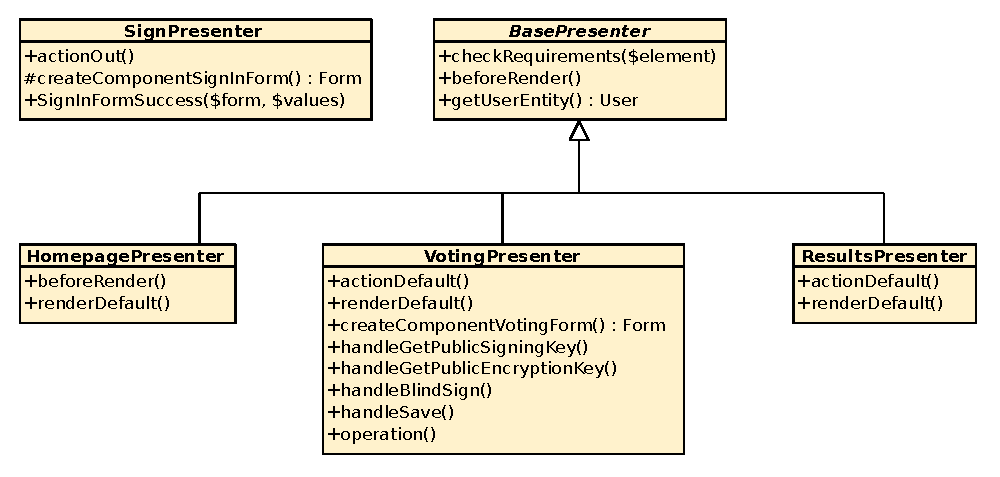
\includegraphics[width=\linewidth]{svg/frontendPresenters.eps}
	\captionsetup{width=\linewidth}
	\caption[Třídy Presenter frontendové části]{Třídy Presenter frontendové části (zdroj: vlastní)}
	\label{fig:FrontendPresenters}
\end{figure}
%--------------%
\clearpage
\paragraph{SignPresenter} Jediným úkolem tohoto presenteru je uživateli poskytnout možnosti přihlášení a odhlášení.

% \tab{popisek}{label}{rozměr (0.0 - 1.0)}{definice sloupců}{obsah} 
\tab{Dostupné akce}{tab:FrontendSignPresenterAction}{1}{c|ccc}{
	\hline
	akce & action* & render* & šablona \\
	\hline
	in & - & - & in.latte \\
	out & actionOut & - & - \\
}

Dostupné akce:
\begin{itemize}
	\item \tt{Sign:in} Zobrazí přihlašovací formulář\\
Nemá definované metody action ani render - ekvivalentní by byly prázdné metody. Jediným úkolem této metody je zobrazit formulář pro přihlášení, který se vytváří metodou \phpinline{SignPresenter::createComponentSignInForm()}. Po~odeslání formuláře se volá opět tato akce, nicméně se provede i callback formuláře \phpinline{SignPresenter::signInFormSuccess()}. V tomto callbacku se aplikace pokusí o přihlášení uživatele pomocí poskytnutých údajů. Presenter je předá třídě implementující rozhraní \phpinline{Nette\Security\IAuthenticator}. Princip přihlašování je popsán v části \ref{section:prihlasovani}. Na tuto akci zároveň odkazují všichni potomci BasePresenter z metody \phpinline{BasePresenter::checkRequirements()}, pokud se uživatel pokusí provést jakoukoli akci jako nepřihlášený (např. po~vypršení session).
	\item \tt{Sign:out} Odhlásí uživatele\\
Uživatel po kliknutí na odkaz ,,Odhlásit'' vyvolá akci tuto akci, kdy je odhlášen a následně přesměrován na přihlašovací formulář -- \tt{Sign:in}. Tato akce nemá render metodu ani šablonu (dochází k přesměrování, které předchází jakémukoli výstupu a ukončuje aktuální cyklus aplikace).
\end{itemize}


%--------------%
\paragraph{BasePresenter} je abstraktní třída, která je společným předkem pro všechny presentery, které jsou dostupné pouze po přihlášení. Také obsahuje metody, které jsou užitečné pro všechny presentery obecně. Vzhledem k tomu, že se jedná o abstraktní presenter, nemá žádné metody action, render ani vlastní šablony. 
Metoda \phpinline{checkRequirements()} slouží k ověření, že je uživatel přihlášen. Rozšiřuje rodičovskou metodu, která detekuje CSRF\footnote{Cross-Site Request Forgery} útoky, je tedy nezbytné zahrnout \phpinline{parent::checkRequirements($element)}%$
. Aby bylo zajištěno správné zobrazení krátkých stavových zpráv \it{flashMessage} a modálních oken během AJAXových požadavků, je zde i metoda \phpinline{beforeRender()}, která se volá vždy před metodami \phpinline{render}.


%--------------%
\paragraph{HomePagePresenter} slouží jako rozcestník po přihlášení uživatele. Jeho jediná akce je \texttt{Homepage:default}, a obsahuje pouze render metodu, která získává objekty Election, které jsou dostupné danému uživateli.


%--------------%
\paragraph{VotingPresenter} je stěžejním presenterem frontendové části aplikace, jejímž prostřednictvím probíhá celý proces volby na straně uživatele. Metoda \phpinline{actionDefault()} získává a \phpinline{renderDefault()}  předává šabloně objekt \phpinline{Election}. Samotný hlasovací lístek je tvořen formulářem. Ten je vytvářen tovární metodou \phpinline{createComponentVotingForm()}. Zde bylo využito \it{generované továrničky}, což je zjednodušený zápis továrních tříd, které pouze vytváří jeden konkrétní objekt. Do~presenteru je pomocí Dependency Injection předána závislost na rozhraní \phpinline{VotingFormFactory} a Nette samo vygeneruje implementaci tohoto rozhraní, které je předáno do Presenteru \cite{Planette}.

Formulář \phpinline{VotingForm} je samostatnou třídou rošiřující \phpinline{Control}\footnote{\Verb{Nette\Application\UI\Control}} - v názvosloví Nette komponentou. Komponenty mohou mít vlastní šablony, což umžňuje zpřehlednit šablonu presenteru pokud není celý formulář vykreslován automaticky přes \phpinline{FormRenderer}. Zároveň je i samotný kód presenteru jednodušší, o vytvoření formuláře, validaci a zpracování se totiž stará třída formuláře.

Hlasovací formulář neobsahuje žádnou logiku pro validaci ani zpracování odeslaných dat. Veškerá validace probíhá pomocí JavaScriptu na straně klienta a data se odesílají teprve po zašifrování a to přímo na presenter pomocí AJAX. Zpracování těchto požadavků (signálů) pomocí handle metod je popsáno v samostatné části~\ref{section:zpracovaniHlasu}~věnované zpracování hlasovacích lístků.


%--------------%
\paragraph{ResultsPresenter} je velice jednoduchý presenter, který opět pomocí metod \phpinline{actionDefault()} a \phpinline{renderDefault()} získá a zpřístupní objekt \phpinline{Election} šabloně k~zobrazení výsledků hlasování / voleb.

%--------------%
%--------------%
\n{3}{Backend}

Tato část obsahuje nástroje pro správu uživatelů, uživatelských oprávnění a~především voleb samotných. Je hojně využíváno formulářů a interaktivních tabulek (neboli datagridů). Formuláře a datagridy jsou samostatné komponenty\footnote{třídy rozšiřující \phpinline{Nette\Application\UI\Control}}. Jednoduché komponenty jsou zpravidla vytvářeny přímo v Presenteru. Složitější chování nebo obsáhlé komponenty je vhodnější oddělit do samostatné třídy. Podrobněji jsou datagridy popsány v části \ref{section:Datagridy}.

Datagridy jsou vytvářeny pomocí třídy \phpinline{App\Backend\Utils\DataGrid\Datagrid}, která zefektivňuje způsob vytváření jednotlivých gridů díky zapouzdření často používaných konstrukcí. Tím se nejen výsledný kód v presenterech zjednoduší, ale zároveň gridy napříč aplikací mají stejné chování a na všechny se aplikuje stejná logika. Tímto přístupem se také podstatně usnadní změny ovlivňující všechny gridy - například změna ikony se projeví všude.

\begin{figure}[h]
	\centering
	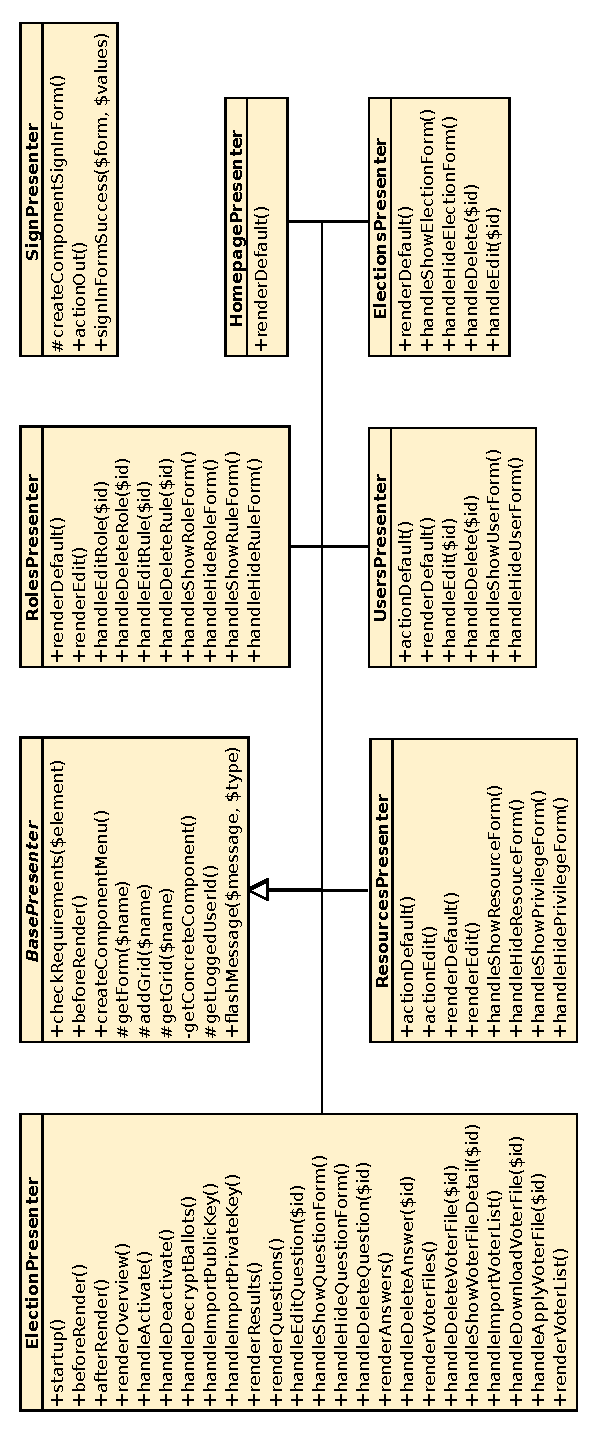
\includegraphics[height=\textheight]{svg/backendPresentersPortrait.eps}
	\captionsetup{width=\linewidth}
	\caption[Třídy Presenter backendové části]{Třídy Presenter backendové části (zdroj: vlastní)}
	\label{fig:BackendPresenters}
\end{figure}

%--------------%
\paragraph{SignPresenter} slouží ke správě přihlášení do aplikace, v zásadě se jedná o obdobu frontendového \phpinline{SignPresenter}. Popis této třídy je tedy identický.


%--------------%
\paragraph{BasePresenter} je stejně jako \phpinline{App\Frontend\Presenters\BasePresenter} abstraktní třídou společnou pro všechny další presentery. Ověřuje, že uživatel je přihlášen a má oprávnění provést požadovanou akci.


%--------------%
\paragraph{HomepagePresenter} hlavní jeho funkcí je umožnit zobrazení navigace po přihlášení i pro uživatele, který nemá definovaná žádná práva a jediné co může v aplikaci provést je se odhlásit. Mohl by zobrazovat i nějakou formu rozcestníku, jako ve frontendové části, to ale obstarává navigační lišta. Dalším vhodným využitím tohoto presenteru by byla prezentace důležitých dat formou \it{dashboardu}.


%--------------%
\paragraph{ElectionsPresenter} poskytuje přehled nad všemi vypsanými volbami, jejich rychlou editaci, mazání a odkaz na zobrazení detailu. Nové volby se také vytváří v tomto presenteru. Při vypisování nových voleb je vhodné zvolit výstižný krátký popisek, jeho editace je uživatelsky přívětivá díky JavaScriptovému pluginu \it{tinyMCE}.


%--------------%
\paragraph{ElectionPresenter} nabízí detailní přehled konkrétních voleb rozdělený do záložek. Některé záložky se zobrazují pouze pokud se volby nacházejí v určitém stavu. Záložka výsledky se například zobrazí až po ukončení voleb. 

V záhlaví detailu se nachází kontextové menu, které umožňuje volby (de)aktivovat, nahrávat seznamy voličů a klíče volební komise. Aktivace voleb způsobí jejich zobrazení voličům, hlasování je umožněno až v řádném termínu. Po aktivaci voleb není možné měnit jejich nastavení, ale lze je opět deaktivovat. Aktivovat a deaktivovat volby lze pouze pokud se nenacházejí v průběhu jejich konání. Po skončení voleb se voličům ukazují pouze výsledky a to do doby než jsou deaktivovány.

Jednotlivými záložkami jsou:
\begin{itemize}
	\item \b{Overview}, kde se zobrazuje formátovaný popis voleb a tři pole s šifrovacími klíči (pokud jsou dostupné). Těmito klíči jsou: privátní a veřejný klíč volební komise a veřejný podpisový klíč serveru.
	\item \b{Results} s výsledky voleb. Tato záložka je distupná pouze po ukončení voleb. V~případě, že dosud nejsou spočítané výsledky, je nabídnuto jejich spočítání a~následně se již zobrazují pouze výsledky v přehledných grafech.
	\item \b{Questions} zobrazí grid otázek definovaných pro dané volby. Otázkou může být volená pozice, její odpověďmi pak jména kandidátů. Při založení nové otázky je možné nastavit minimální a maximální počet otázek, zda je odpověď povinná a~jednotlivé odpovědi. V gridu je možné otázky editovat a mazat.
	
	\item \b{Answers} obsahuje grid všech odpovědí, které byly definované při zakládání otázek, zde je možné odpovědi mazat.
	
	\item \b{Voter list} zobrazí grid s aktivním seznamem voličů.
	
	\item \b{Voter files} v tomto gridu se nachází všechny soubory se seznamem voličů, které byly pro dané volby nahrány. Soubory je možno prohlížet, mazat, stáhnout a~aplikovat vybraný soubor jako aktivní seznam voličů. Nový soubor lze nahrát přes kontextové menu v záhlaví.
	
\end{itemize}

%--------------%
\paragraph{UsersPresenter} jednoduchý presenter s gridem uživatelů a formulářem pro přidávání / editaci uživatelů. Formulář umožňuje uživatelům přidělovat role i změnit heslo. Aplikace neobsahuje žádný registrační formulář, nové uživatele musí vždy přidávat osoba s patřičným oprávněním - pravděpodobně administrátor aplikace. Jak bylo popsáno v části \ref{section:prihlasovani}, není potřeba zakládat uživatelské účty voličům, ale pouze osobám, kterým je potřeba navýšit oprávnění.

%--------------%
\paragraph{RolesPresenter} výchozí View tohoto presenteru nabízí grid všech dostupných rolí a~formulář pro jejich základní editaci. Pomocí akce gridu je možné zobrazit detail role, kde se nachází seznam definovaných pravidel přístupu ve formě gridu. Tato pravidla lze editovat, mazat a přidávat nová.

%--------------%
\paragraph{ResourcesPresenter} velice podobý předchozímu RolePresenter. Tento umožňuje správu prostředků (\textit{Resource}), na stránce detailu je pak k dispozici správa akcí (\textit{Privilege}) dostupných pro daný prostředek.

\n{3}{Core}
Tento modul je společný pro frontendovou i backendovou část a obsahuje pouze uživatelsky přívětivé zpracování chybových stavů. Pokud se uživatel pokouší přistoupit na neexistující stránku, není nalezen požadovaný záznam v databázi (HTTP~404) nebo nemá uživatel potřebná oprávnění k zobrazení stránky (HTTP~403), místo základních chybových stránek HTTP serveru mu je zobrazena chybová stránka vygenerovaná Nette. Stejně tak v případě chyby serveru (HTTP~500). 

V případě, že se Nette nachází ve vývojovém režimu, jsou všechny chyby aplikace předávány ke zpracování nástroji Tracy (dříve Laděnka) \cite{Tracy}, který vypíše chybu včetně části zdrojového kódu, předávaných proměnných, dotazů na databázi a dalších velice užitečných informací pro ladění chyb. V produkčním režimu jsou chyby předávány \texttt{ErrorPresenteru}, který chyby 4xx předává dále do \texttt{Error4xxPresenter} případně rovnou předá statickou šablonu s chybou 500 nebo 503.



\n{2}{Zpracování hlasovacích lístků} \label{section:zpracovaniHlasu}

\n{2}{Další části aplikace}

\n{3}{Datagridy} \label{section:Datagridy}
Zkráceně gridy, tyto interaktivní tabulky umožňují kromě zobrazení dat i jejich filtraci, stránkování, akce nad řádkem tabulky (např. odkaz směřující na Signál) a mnoho dalších funkcí. Gridy přijímají data jako objekt \phpinline{Datasource}, který může obsahovat data ve formě obyčejného pole nebo dotazu SQL \cite{ContributteDataGrid}. Kromě jednoho případu v této aplikaci vždy pracují s SQL dotazem. Výhoda tohoto přístupu je minimalizování potřebného objemu dat k zobrazení gridu. Po změně filtrace nebo stránky je vždy upraven SQL dotaz a až následně odeslán na databázový server, filtrace a stránkování tedy probíhá přímo na SQL serveru, nikoli pomocí PHP nebo JavaScriptu.

Akce nad řádkem jsou typicky úlohy typu editace, mazání zobrazení detailu a směřují na Signál presenteru (metody handle). Jsou reprezentovány ikonami. Požadavek na vymazání řádku (záznamu) je navíc opatřen potvrzovacím dialogovým oknem, aby nedošlo k nechtěnému smazání při nechtěném kliknutí.


% ============================================================================ %
\nn{Závěr}
Text závěru.

% ============================================================================ %

